\documentclass{article}
\usepackage{setspace}
\usepackage{amsmath}
\usepackage{amssymb}
\usepackage{amsthm}
\usepackage{graphicx} 
\usepackage{float} 
\usepackage{fancyhdr}                                
\usepackage{lastpage}        
\usepackage{textcomp}                               
\usepackage{layout}   
\usepackage{subfigure} 
\pagestyle{fancy}  
\lhead{ZHANG HUAKANG}
\chead{Assignment 1} 
\rhead{DB92760} 
\renewcommand{\baselinestretch}{1.05}
\title{Assignment 1 of CISC 1006}
\author{ZHANG HUAKANG \\ DB92760 \\ \\ CPS, FST}
\begin{document}
    \maketitle
    \section{}
            \paragraph{
                \begin{tabular}{c|c|c}
                    \hline
                    1 &H &H \\
                    &H & T\\
                    & T&H \\
                     & T&T \\
                    \hline
                    2 & H& \\
                     & T& \\
                    \hline
                    3&H &H \\
                    & H&T \\
                    & T&H \\
                    & T&T \\
                    \hline
                    4&H & \\
                    &T & \\
                    \hline
                    5&H &H \\
                    & H&T \\
                    & T&H \\
                    & T&T \\
                    \hline
                    6&H & \\
                    &T & \\
                    \hline
                \end{tabular}
            }
        \subsection{}
            \paragraph{
                $$A=\{1HH,1HT,1TH,1TT,2H,2T\}$$
            }
        \subsection{}
            \paragraph{
                \begin{equation*}
                    \begin{split}
                        B=\{& 1HH,1HT,1TH,1TT,\\
                            &3HH,3HT,3TH,3TT,\\
                            &5HH,5HT,5TH,5TT\}\\
                    \end{split}
                \end{equation*}
            }
        \subsection{}
            \paragraph{
                \begin{equation*}
                    \begin{split}
                        A'=\{& 4H,4T,6T,6H,\\
                            &3HH,3HT,3TH,3TT,\\
                            &5HH,5HT,5TH,5TT\}\\
                    \end{split}
                \end{equation*}
            }
        \subsection{}
            \paragraph{
                \begin{equation*}
                    \begin{split}
                        A'\cap B =\{&3HH,3HT,3TH,3TT,\\
                            &5HH,5HT,5TH,5TT\}\\
                    \end{split}
                \end{equation*}
            }
        \subsection{}
            \paragraph{
                \begin{equation*}
                    \begin{split}
                        A'\cup B =\{&1HH,1HT,1TH,1TT,\\
                            &2H,2T\\
                            &3HH,3HT,3TH,3TT,\\
                            &5HH,5HT,5TH,5TT\}\\
                    \end{split}
                \end{equation*}
            }
    \section{}
        \subsection{}
            \begin{figure}[H]
                \centering
                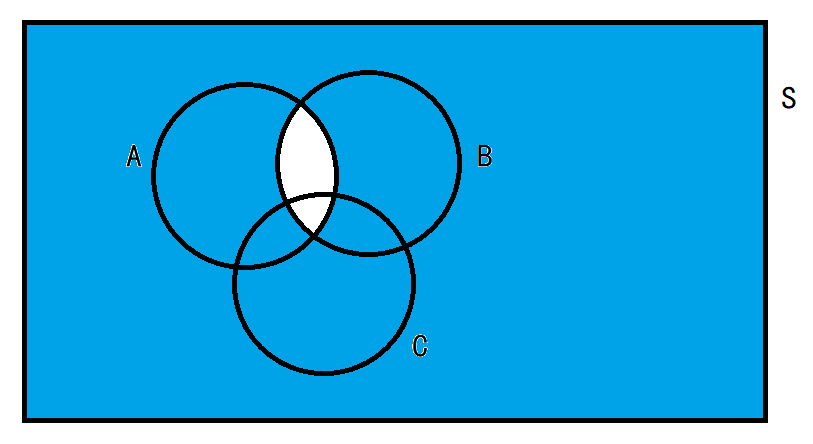
\includegraphics[width=0.9\textwidth]{img/Assignment1-01.png}
            \end{figure}
        \subsection{}
            \begin{figure}[H]
                \centering
                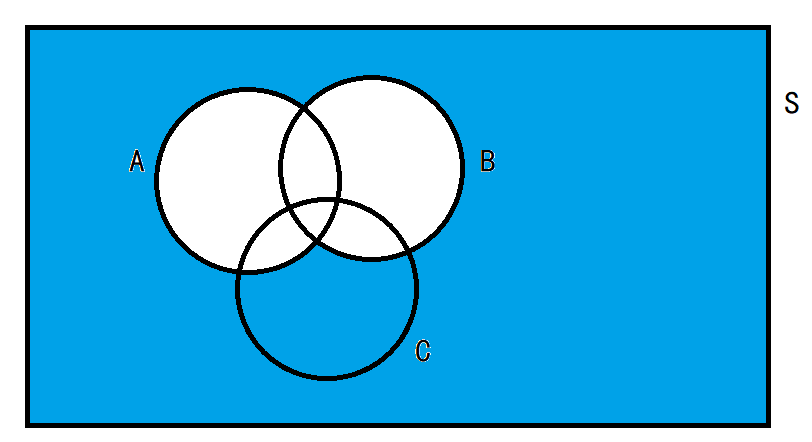
\includegraphics[width=0.9\textwidth]{img/Assignment1-02.png}
            \end{figure}
        \subsection{}
            \begin{figure}[H]
                \centering
                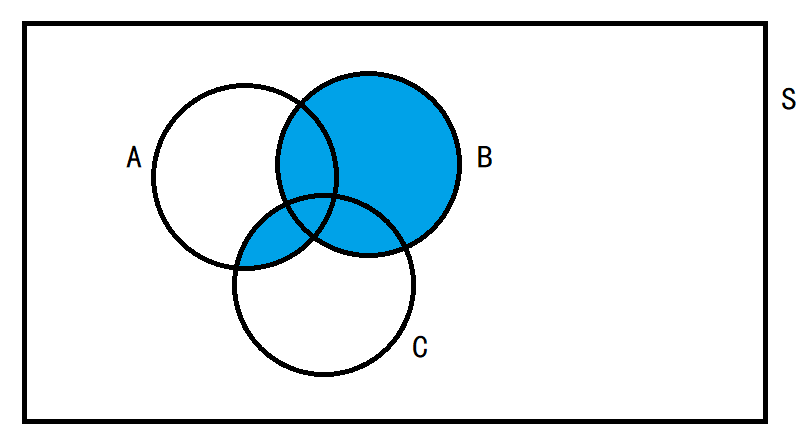
\includegraphics[width=0.9\textwidth]{img/Assignment1-03.png}
            \end{figure}
    
    \section{}
        \subsection{}
            \paragraph{
                $$P_6^6=720$$
            }
        \subsection{}
            \paragraph{
                $$P_4^4P_3^3=144$$
            }
        \subsection{}
            \paragraph{
                $$P_4^4P_5^2=480$$
            }
        \subsection{}
            \begin{itemize}
                \item $[1,4,4]$, $C_9^1C_8^4C_4^4=630$
                \item $[1,3,5]$, $C_9^1C_8^3C_5^5=504$
                \item $[2,2,5]$, $C_9^2C_7^2C_5^5=756$
                \item $[2,3,4]$, $C_9^2C_7^3C_4^4=1260$
                \item $[2,4,3]$, $C_9^2C_7^4C_3^3=1260$
            \end{itemize}
            $$Total= 4410$$
    \section{}
        \subsection{}
            \paragraph{
                $$C_5^4=5$$
            }
        \subsection{}
            \paragraph{
                $$C_5^1C_7^3=175$$
            }
        \subsection{}
            \paragraph{
                $$C_5^1C_7^3+C_5^2C_7^2+C_5^3C_7^1+C_5^4C_7^0=460$$
            }
        \subsection{}
            \paragraph{
                $$C_5^0C_7^4+C_5^1C_7^3+C_5^2C_7^2=420$$
            }

\end{document}